\begin{figure}[ht!]
	\begin{subfigure}{\linewidth}
		\caption{}
		\centering
		% include second image
		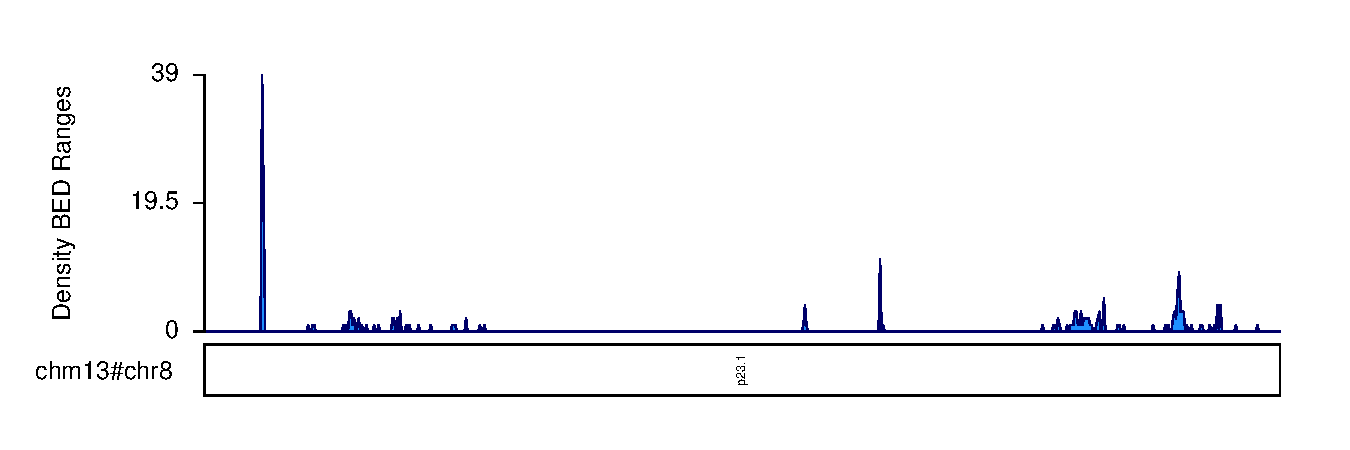
\includegraphics[width=1.0\linewidth, trim=0cm 2.75cm 0cm 0cm]{fig/tips/chr8_chm13_beta_defensin_locus_odgi_tips_w50000_karyoploteR}
		\label{fig:tips-karyo}
	\end{subfigure}
	%	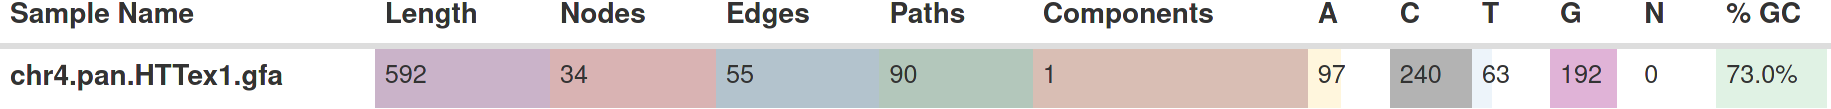
\includegraphics[width=\linewidth]{fig/metrics/chr4.pan.HTTex1.gfa.multiqc_odgi_stats.png}
	\caption{Visualizing the contigs of a beta-defensin locus pangenome graph. (\textbf{a}) Breakpoint ranges of the contigs in the beta-defensin locus pangenome graph of 90 haplotypes relative to CHM13. The \textit{odgi tips} results are visualized as the density of BED ranges across the whole \textit{p23.1} cytoband. The high peak at the beginning of \textit{p23.1} indicates that 39 contigs of the graph broke there relative to CHM13. (\textbf{b}) \FIXME{ADD VIZ AS SOON AS THE SORTING IS FINISHED.}}
	\label{fig:tips}
\end{figure}
